\documentclass{article}

\usepackage[dark,showauthor]{../../../classes/dim}

\begin{document}
    \header{Introduction to Optimization}{Homework 1}

    \begin{tasks}
        \item \begin{enumerate}
            \item Let \(n=1,\ S=[0, \infty)\subset\R{1},\ C=[1, \infty)\subset S,\ f(x)=x^2\). \(f(x)\) attains its minumum but not the maximum.
            \item \begin{enumerate}
                \item Let \(n=1,\ S=(0, 2),\ C=(0, 1),\ f(x)=x\).
                \item Let \(n=1,\ S=(0, 2),\ C=(0, 1),\ f(x)=-x(x-2)\).
            \end{enumerate}
        \end{enumerate}
        \item \begin{enumerate}
            \item The plots: \\
                \begin{minipage}{0.9\linewidth}
                    \centering
                    \begin{minipage}[t]{0.49\linewidth}
                        \begin{figure}[H]
                            \centering
                            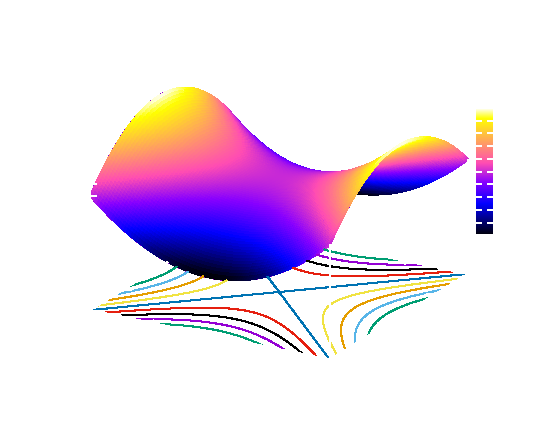
\includegraphics[width=1\linewidth]{1-2-a-1.eps} 
                            \caption[\(f\)]{plot of \(f\)}
                        \end{figure}
                    \end{minipage}      
                    \begin{minipage}[t]{0.49\linewidth}
                        \begin{figure}[H]
                            \centering
                            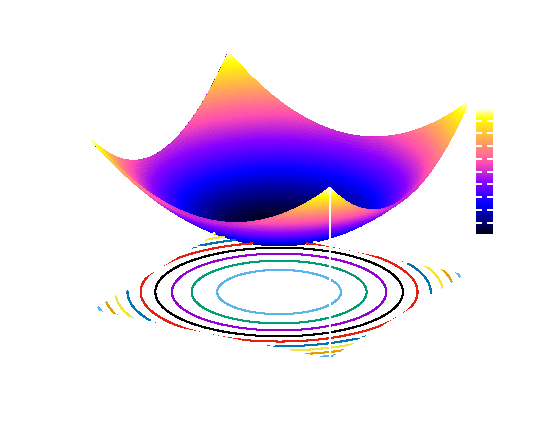
\includegraphics[width=1\linewidth]{1-2-a-2.eps}
                            \caption[\(g\)]{plot of \(g\)}
                        \end{figure}
                    \end{minipage}
                \end{minipage}
            \item Since \(D\) is not closed, \(f\) doesn't attain either 
                  a minumum or a maximum but g attains a minimum at \((0, 0)\) (very clear form the plot):
                  \begin{displaymath}
                    \nabla g(x, y) = \langle 2x, 2y\rangle,\ 
                    \nabla g(0, 0) = \langle 0, 0\rangle
                  \end{displaymath}
            \item Now, since \(\bar{D}\) is closed, out of continuity of \(f\) 
                  and \(g\), both attain both, a minumum and a maximum:
                  \begin{displaymath}
                    \begin{aligned}
                        \max_{x\in\bar{D}} f(x) &= 1, & x &= \langle \pm1, 0\rangle \quad \quad & 
                        \max_{x\in\bar{D}} g(x) &= 1, & x &= \langle \cos\alpha, \sin\alpha\rangle \forall \alpha \in [-, 2\pi] \\
                        \max_{x\in\bar{D}} f(x) &= -1, & x &= \langle 0, \pm1\rangle &
                        \max_{x\in\bar{D}} g(x) &= 0, & x &= \langle 0, 0\rangle \\
                    \end{aligned}
                  \end{displaymath}
        \end{enumerate}
        \item \begin{enumerate}
            \item Since all eigenvalues are \(\geq 0\) the matrix is \textit{positive semidefinite}.
            \begin{displaymath}
                \begin{aligned}
                    \det(M-\lambda I)
                    &= (2-\lambda)^3 - 2 - 3(2-\lambda) & \\
                    &= -\sigma^3-2+3\sigma & \sigma&\equiv\lambda-2 \\
                    &= -(\sigma-1)^2(\sigma+2) & \sigma &= -2, 1 \implies \boxed{\lambda = 0, 3} \\
                    &= 0 
                \end{aligned}
            \end{displaymath}
            \item Since all eigenvalues are \(> 0\) the matris is \textit{positive definite}
            \begin{displaymath}
                \begin{aligned}
                    \det(M-\lambda I)
                    &= (2-\lambda)^3 - 3(2-\lambda) + 2 & \\
                    &= -\sigma^3 + 3\sigma + 2 & \sigma&\equiv\lambda-2 \\
                    &= (\sigma + 1)^2(\sigma - 2) & \sigma&=-1, 2 \implies \boxed{\lambda=1, 4}
                \end{aligned}
            \end{displaymath}
            \item Since all eigenvalues are \(> 0\) the matris is \textit{positive definite}
            \begin{displaymath}
                \begin{aligned}
                    \det(M-\lambda I)
                    &= (1-\lambda)(5-\lambda)(9-\lambda)+48-16(1-\lambda)-9(5-\lambda)-4(9-\lambda) & \\
                    &= -\lambda(\lambda^2 - 15\lambda + 30) \\
                    &= 0 \implies \boxed{\lambda = 0, \frac{15 - \sqrt{105}}{2}, \frac{15 + \sqrt{105}}{2}}
                \end{aligned}
            \end{displaymath}
        \end{enumerate}
        \item \begin{enumerate}
            \item Since \(f\) is just the distance function from \(Ax\) to \(b\) squared, 
                  we can say that when \(Ax = b\) the distance will be minimized. To find
                  such \(x\) we can write:
                  \begin{displaymath}
                    x = A^\dagger b = R^{-1}Q^Tb
                  \end{displaymath}
            \item Let's rewrite \(f\) as such: 
                  \begin{displaymath}
                    f(x_1, \dots, x_n) = \sum_{i=1}^m \frac{1}{2} \left(\sum_{j=1}^n x_j \cdot a_{ij} - b_i\right)
                  \end{displaymath}
                  and then
                  \begin{displaymath}
                    \begin{aligned}
                        H_f(x) 
                        &= \left(\frac{\delta^2f(x)}{\delta x_i\delta x_j} \right)_{i,j = 1,\dots,n} \\
                        &= \left(\frac{\delta}{\delta x_i}\cdot\frac{\delta f(x)}{\delta x_j}\right)_{i,j = 1,\dots,n} \\
                        &= \left(\frac{\delta}{\delta x_i}\cdot\left(\sum_{p=1}^m a_{pj} \left(\sum_{q=1}^n x_q \cdot a_{pq} - b_p\right)\right)\right)_{i,j = 1,\dots,n} \\
                        &= \left(\sum_{p=1}^n a_{pj} \cdot a_{pi}\right)_{i,j = 1,\dots,n} \\
                        &= A^TA \\
                        x^T (A^T A) x &= \langle Ax,Ax\rangle \ge 0 \Longleftrightarrow A^T A \text{ positive semidefinite}
                    \end{aligned}
                  \end{displaymath} 
                  if \(A\) is injective, \(Ax = 0 \implies x = 0\), then 
                  \(\langle Ax, Ax\rangle = 0 \implies x = 0\), therefore 
                  \(\langle Ax, Ax\rangle > 0 \ \forall \ x \ne 0 \)
            \item let
                  \begin{displaymath}
                    A = \mat{\xi_1 & \dots & \xi_m \\ 1 & \dots & 1}^T,\
                    b = \mat{\eta_1 & \dots & \eta_m}^T,\
                    x = \mat{x_1 & x_2},\
                    g(y) = x_1\cdot y + x_2
                  \end{displaymath}
                  then \(\bar{x}\) which minimizes \(f\) will also minimize \(\sum_{i=1}^m (g(\xi_i) - \eta_i)^2\).
                  Since \(H_f = A^TA\) we get that 
                  \begin{displaymath}
                    H_f = \mat{\sum\limits_{i=1}^m \xi_i^2 & \sum\limits_{i=1}^m \xi_i \\ \sum\limits_{i=1}^m \xi_i & m}.
                  \end{displaymath}
                  \begin{proof}\footnote{a friend helped me with this one.}
                    Since \(A^TA\) is always positive semi-definite, what's left to show is 
                    that it's invertible only when there are at least one pair of \(i \ne j\) 
                    where \(\xi_i \ne \xi_j\).
                    \footnotesize
                    \begin{displaymath}
                        \begin{aligned}
                            \det(H_f) 
                            &= m\sum\limits_{i=1}^m \xi_i^2 - \left(\sum\limits_{i=1}^m \xi_i\right)^2 \\
                            &= \sum\limits_{j=1}^m\sum\limits_{i=1}^m \xi_i^2 - \sum\limits_{j=1}^m\xi_j\sum\limits_{i=1}^m \xi_i \\
                            &= \frac{1}{2}\sum\limits_{j=1}^m\sum\limits_{i=1}^m \xi_i^2 + \frac{1}{2}\sum\limits_{j=1}^m\sum\limits_{i=1}^m \xi_j^2 - \sum\limits_{j=1}^m\sum\limits_{i=1}^m \xi_i\xi_j \\
                            &= \frac{1}{2}\sum\limits_{j=1}^m\sum\limits_{i=1}^m \left(\xi_i^2 + \xi_j^2 - 2\xi_i\xi_j\right) \\
                            &= \frac{1}{2}\sum\limits_{j=1}^m\sum\limits_{i=1}^m (\xi_i - \xi_j)^2
                        \end{aligned}
                    \end{displaymath}
                    Since \((\xi_i-\xi_j)^2\) is always \(\ge 0\), \(\det(H_f) = 0 \Longleftrightarrow (\xi_i-\xi_j)^2 = 0\ \forall\ i,j \Longleftrightarrow \xi_i = \xi_j\ \forall\ i,j\).
                  \end{proof}
                \end{enumerate}
        \item \begin{enumerate}
            \item By definition of totaly differentiability
                  \begin{displaymath}
                    \begin{gathered}
                        f(x + d) = f(x) + \nabla f(x)^T d + o(\|d\|) \quad \text{for } \|d\| \to 0 \\ 
                        \Downarrow \\
                        f(x + d) - f(x) = \nabla f(x)^T d + o(\|d\|) \quad \text{for } \|d\| \to 0
                    \end{gathered}
                  \end{displaymath}
            \item By Taylor expansion if \(f: \R{n} \to \R{}\) is two times continiuously 
                  differentiable 
                  \begin{displaymath}
                    \begin{gathered}
                        f(x + h) = f(x) + \nabla f(x)^T h + {\color{tcum}\frac{1}{2}h^T H_f(x)h + o(\|h\|^2)} \\
                        \Downarrow \\
                        f(x + h) - f(x) = \nabla f(x)^T h + {\color{tcum}\frac{1}{2}h^T H_f(x)h + o(\|h\|^2)} \\
                        \Downarrow \\
                        f(x + h) - f(x) = \nabla f(x)^T h + {\color{tcum}O(\|h\|^2)} \\
                    \end{gathered}
                  \end{displaymath}
            \item By Taylor expansion if \(f: \R{n} \to \R{}\) is two times continiuously 
                  differentiable 
                  \begin{displaymath}
                    \begin{gathered}
                        f(x + h) = f(x) + \nabla f(x)^T h + \frac{1}{2}h^T H_f(x)h + o(\|h\|^2) \\
                        \implies \\
                        f(x + h) - f(x) = \nabla f(x)^T h + \frac{1}{2}h^T H_f(x)h + o(\|h\|^2)
                    \end{gathered}
                  \end{displaymath}
        \end{enumerate}
        \item \begin{multicols}{2}
            \begin{enumerate} \footnotesize
            \item Compatibility:
                  \begin{displaymath}
                    \begin{aligned}
                        &&\|Ay\| &\le \|A\| \cdot \|y\| \\
                        &\implies&\|A\| &\ge \frac{\|Ay\|}{\|y\|} & \text{ for } \|y\| \ne 0 \\
                        &\implies&\|A\| &\ge \left\|A\frac{y}{\|y\|}\right\| & \text{ for } \|y\| \ne 0 \\
                        &\implies&\|A\| &\ge \left\|Ay\right\| & \text{ for } \|y\| = 1 \\
                        &\implies&\|A\| &= \max_{\|y\| = 1} \|Ay\|
                    \end{aligned}
                  \end{displaymath}
            \item Sub-multiplicativity\footnote{\url{https://math.stackexchange.com/questions/435621/show-that-the-operator-norm-is-submultiplicative}}:
                  \begin{displaymath}
                    \begin{aligned}
                        ||AB|| 
                        &= \max_{x \ne 0} \frac{||ABx||}{||x||} \\
                        &= \max_{Bx \ne 0}\frac{||ABx|| }{||x||} \\
                        &= \max_{ Bx\ne 0}\frac{||ABx||}{||Bx||} \frac{||Bx||}{||x||} \\
                        &\le \max_{y \ne 0} \frac{||Ay||}{||y||} \max_{x \ne 0} \frac{||Bx||}{||x||}
                    \end{aligned}
                  \end{displaymath}
                  \footnotesize
        \end{enumerate}\end{multicols}
    \end{tasks}
\end{document}